\chapter{Test Setup}
\label{chap:\currfilebase}

\section{Specimen}
\begin{figure}[!ht]
    \centering
    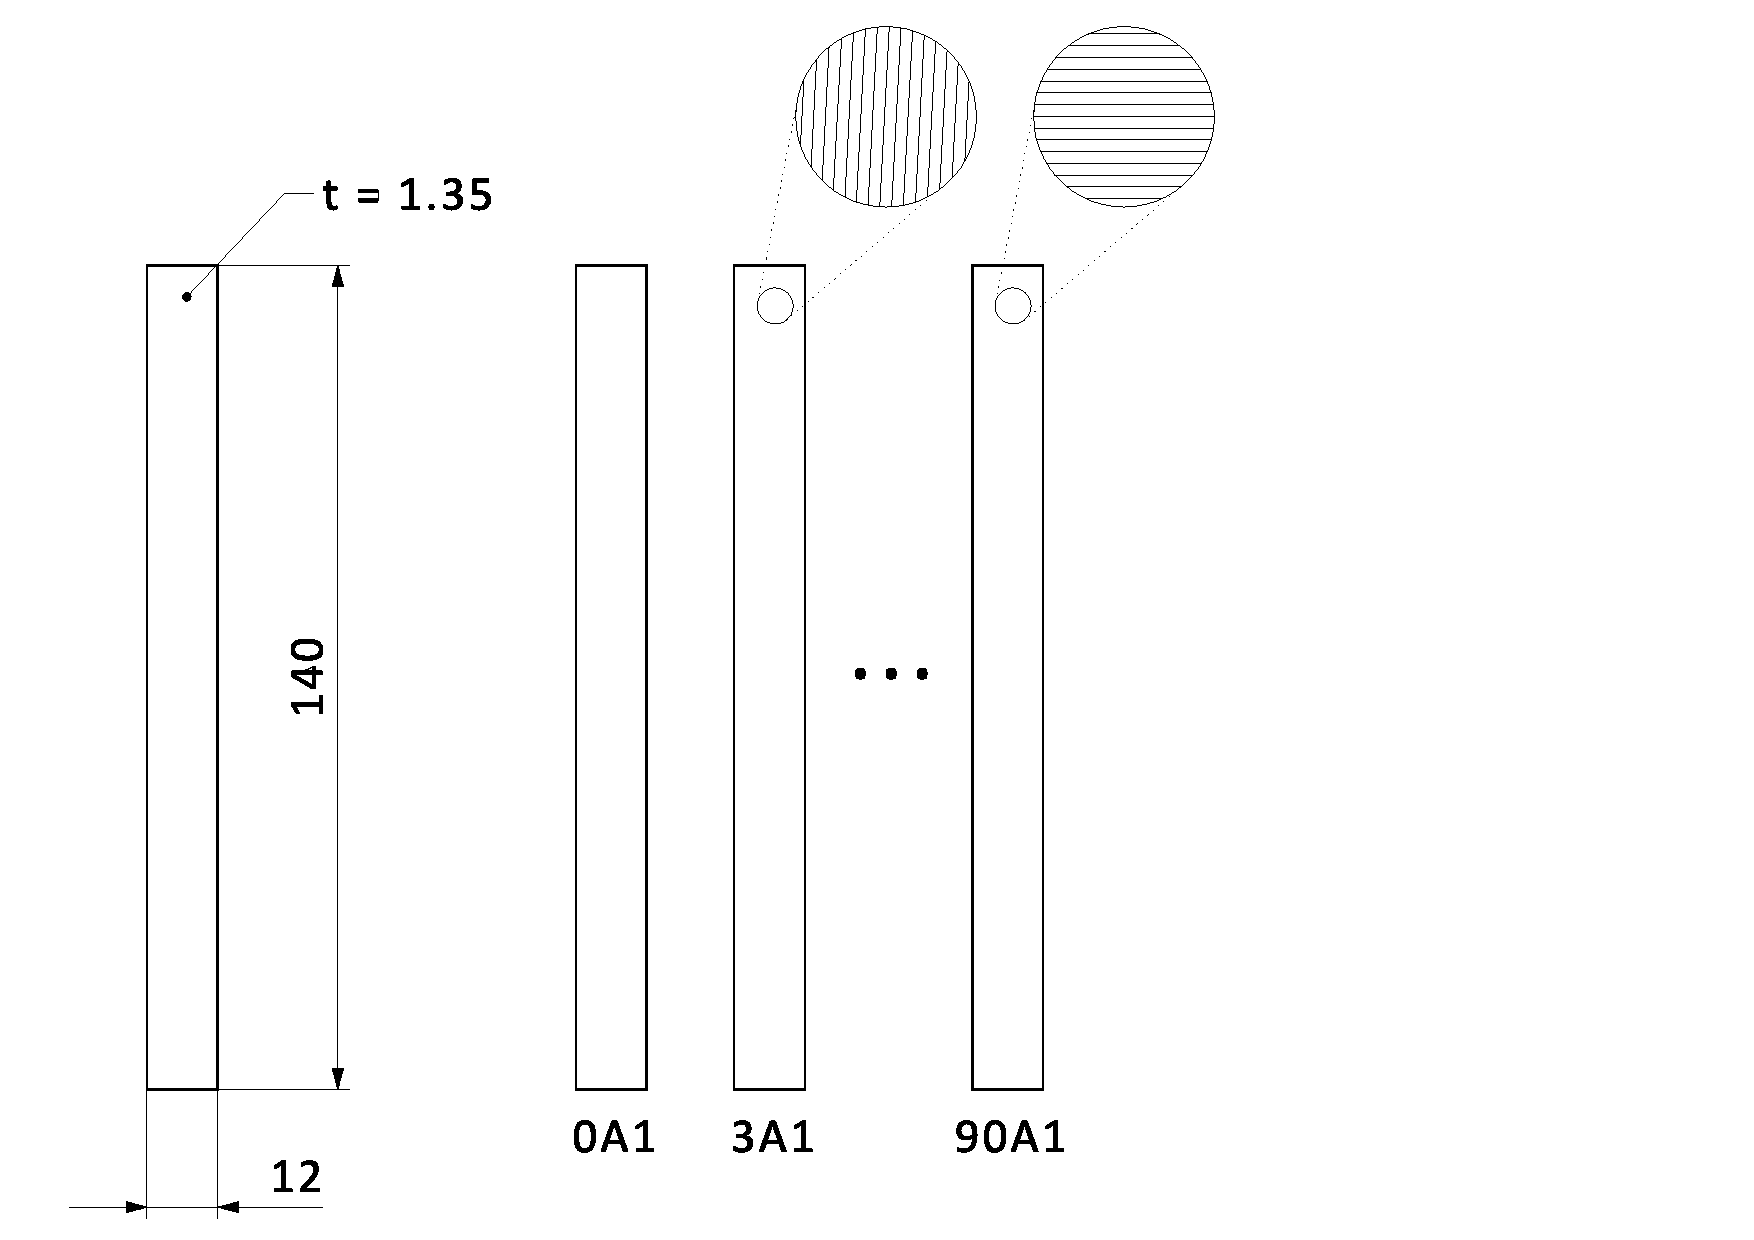
\includegraphics[scale=0.4]{\imgpath/\currfilebase/Specimen_nx_dim_labels.pdf}
    \caption{Specimen dimensions and different fiber orientations}
    \label{fig:Specimen_nx_dim_labels}
\end{figure}
\begin{figure}[!ht]
    \centering
    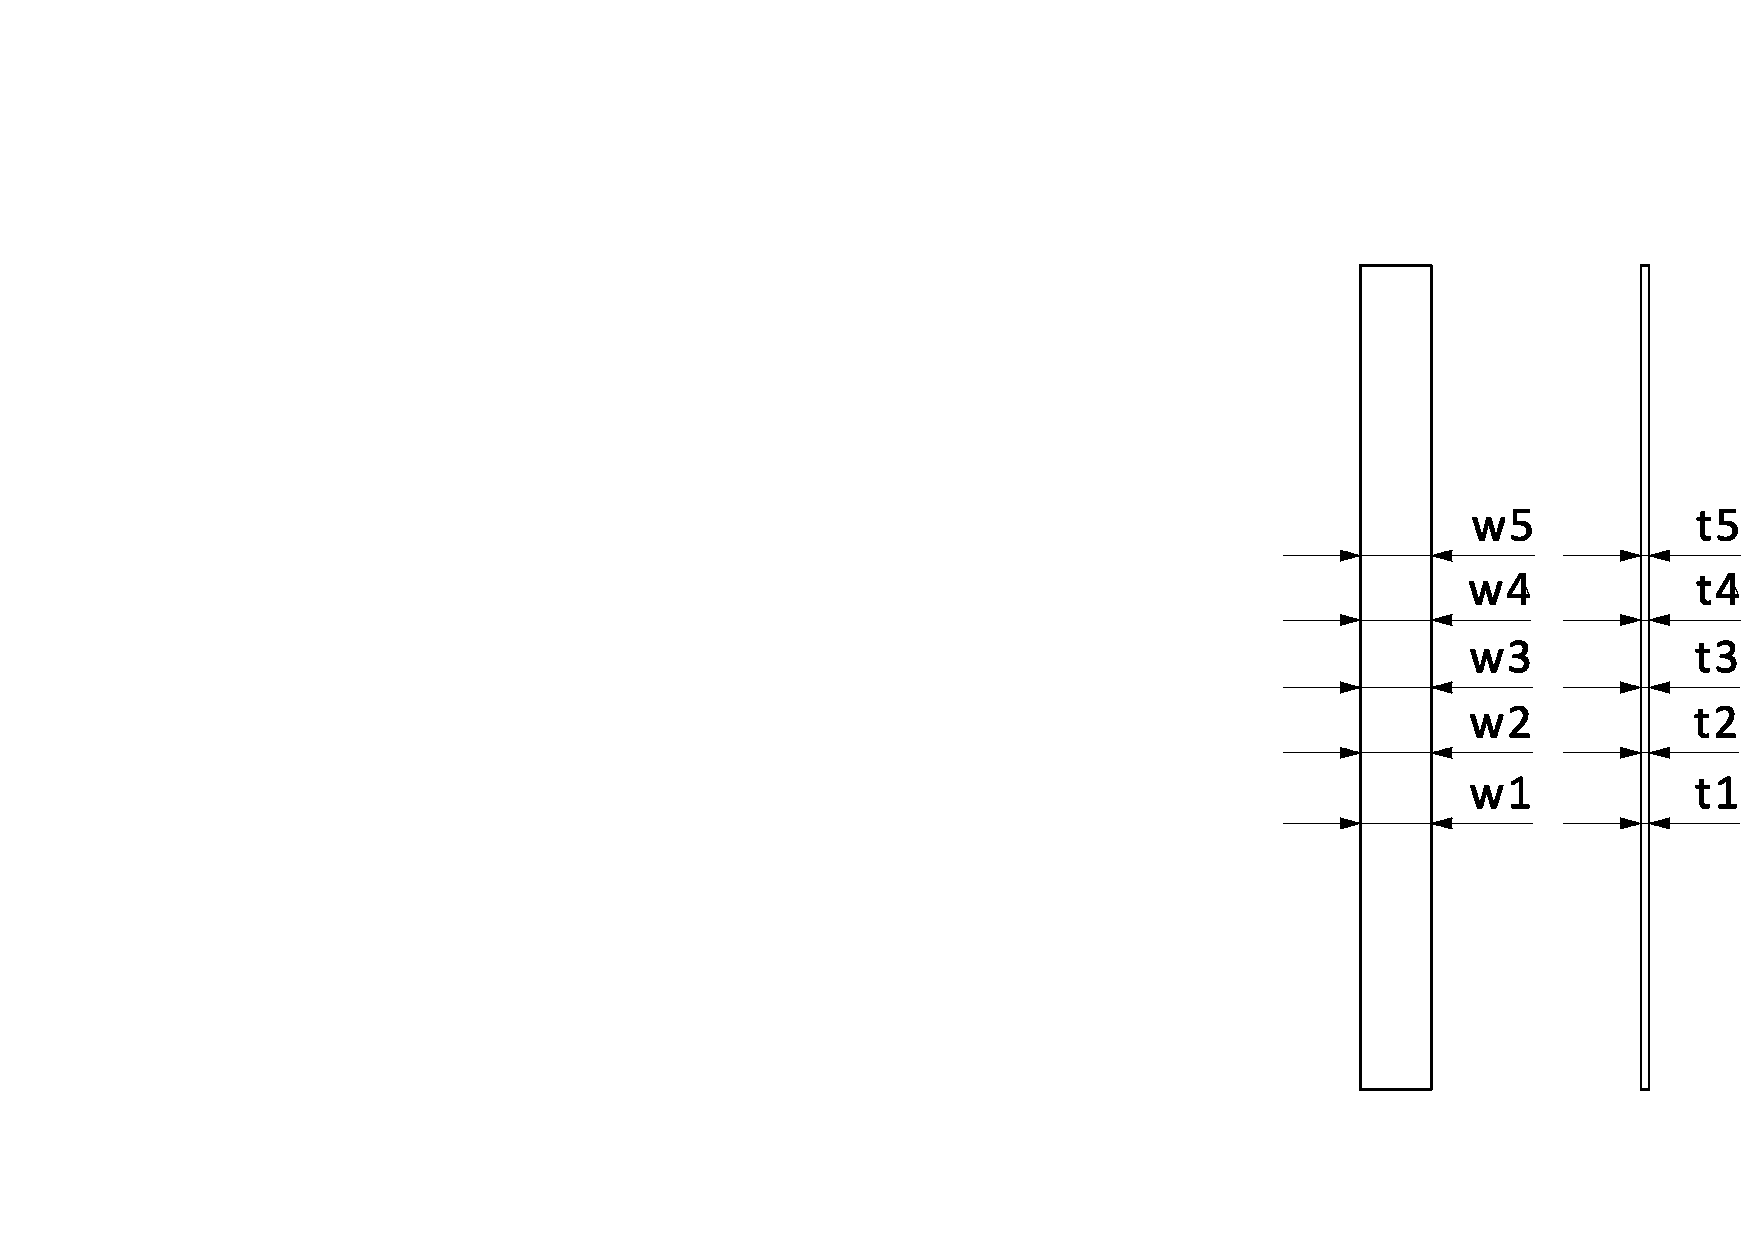
\includegraphics[scale=0.4]{\imgpath/\currfilebase/Specimen_nx_meas.pdf}
    \caption{Specimen dimension measurements}
    \label{fig:Specimen_nx_meas}
\end{figure}

% A phenomenological model aims to describe the time dependant value of an unknown variable using mathematical relations to other, continuously measured variables solely. Thus there is namely no physical connection between the described and the measured data needed.
% The mathematical model mentioned is approached as a first order differential equation
% \begin{align}
%   \frac{\mathrm{d}y}{\mathrm{d}t}	&= p_0+p_1\cdot y(t) +p_2\cdot u_1(t) +\dots + p_n\cdot u_{n-1}(t) \label{eqn:pt1func}
% \end{align}
% where the zero balancing parameter $p_0$, the time lag parameter $p_1$ and the sensitivity parameters $p_i$ of the input values $u_{i-1},i\in\{\mathbb{N}|2\dots n\}$ are to be adjusted to fit the variable $y$ best. This curve fitting is achieved using a least square method during times where both the variable to be described and the input values are known. A prognosis of the $y$ value may be done iteratively every time step of equal length when all input values are updated.
% \begin{align}
%   y(t)  &= y(t-\Delta t)+\frac{\Delta y}{\Delta t}\big(y(t),u_1(t),\dots,u_{n-1}(t)\big)\cdot\Delta t \\
%   y(t)	&= y(t-\Delta t)+\Big[p_0+p_1\cdot y(t-\Delta t)+p_2\cdot u_1(t)+\dots p_n\cdot u_{n-1}(t)\Big]\cdot \Delta t \label{eqn:pt1funciter}
% \end{align}
% where $\Delta t$ is small enough that $\frac{\Delta y}{\Delta t}\big(y(t-\Delta t),u_1(t),\dots,u_{n-1}(t)\big) \approx\frac{\Delta y}{\Delta t}\big(y(t),u_1(t),\dots,u_{n-1}(t)\big)$.\par
% In the case of this thesis the variable to be described is the relative positioning error motion with respect to the first deviation. The measured temperatures may be used as continuously measured variables since their measurement is possible during productive MT applications. The relative positioning error motion however can only be known during measurement tests which implies that MT down time is needed for curve training sets when using the phenomenological model as deviation compensation tool. As mentioned, the least square method is used for curve fitting during training sets.\par
% In Figure~{\ref{fig:pt1model}} the phenomenological model of a short warm-cold test is applied where the curve training sets make up approximately one fourth of the overall machine tool application indicating the quality of the phenomenological model using Equation~{\ref{eqn:pt1funciter}}. 

% \begin{figure}[!ht]
% \centering
% \includegraphics[width=0.8\linewidth]{figures/phenomenologicalmodel/example/pt1model}
% \caption[Phenomenological model of the warm-cold test 10112017a]{Phenomenological model of the first target point in the warm-cold test 10112017a (see Figure~{\ref{fig:warmcoldtest_10112017a_devtemp}}), using Equation~{\ref{eqn:pt1funciter}} as model function, the mean temperatures over the individual measurement sequences of the listed listed sensors as input variables $u_{i-1}$ and the relative positioning error motion $\text{EYY}_1(t)\!-\!\text{EYY}_1(0)$ as value to be described $y$.}
% \label{fig:pt1model}
% \end{figure}

% When applying the model with a longer test set duration the curve fit will improve. But using the model for compensation on the basis of one test set only is dangerous since varying environmental condition may cause a wrong weighting on the different input variables $u_i$. In Figure~{\ref{fig:pt1model2}}) for example additional deflections are induced to the positioning error motion by the warm-up phase of the MT causing the deflection pattern of the first warm-cold sequence to differ from the second. When fitting the curve during a test set in the first sequence the sensitivity parameters $p_i$ may depict the second phase with adequate accuracy only when the initial values $p_i(t=0)$ are chosen in the correct range. In all other cases the least square fit algorithm will adjust the sensitivity parameters at a local minimum that allows the model to fit the curve well in the first sequence but does not suffice in the second. The number of local minima declines if more measurement data is gathered and implemented to the model since less possible sensitivity parameter combinations may fit the data provided. This in return expands the range the initial values may be chosen in for the least square fit to approximate best depiction.

% \begin{figure}[!ht]
% \centering
% \includegraphics[width=0.8\linewidth]{figures/phenomenologicalmodel/example/pt1model2}
% \caption[Phenomenological model of the warm-cold test 23112017]{Phenomenological model of the first target point in the warm-cold test 23112017 (see Figure~{\ref{fig:warmcoldtest_23112017_devtemp}}), using Equation~{\ref{eqn:pt1funciter}} as model function, the mean temperatures over the individual measurement sequences of the listed listed sensors as input variables $u_{i-1}$ and the relative positioning error motion $\text{EYY}_1(t)\!-\!\text{EYY}_1(0)$ as value to be described $y$.}
% \label{fig:pt1model2}
% \end{figure}

%-----------------------------------------------------